\documentclass[twocolumn]{article}

\renewcommand*{\arraystretch}{1.5}
\usepackage{pgfplots}
\usepackage{array}
\usepackage{amssymb}
\usepackage{tikz}
\usepackage{lettrine}
\usepackage{fix-cm}
\usepackage[latin1]{inputenc}
\usepackage{etoolbox}
 \usepackage[a4paper,vmargin={20mm,20mm},hmargin={20mm,10mm}]{geometry}
 
\title{COMP41450 - Assignment}
\author{Kevin Heffernan - \textbf{ID: 11277955}}
\date{}

\begin{document}
\maketitle

\lettrine[lines=5,slope=-0pt,nindent=-0pt]{I}{\textbf{ntroduction}}\ \ \ \ For my neural network, I have chosen to use the suggested backpropagation 
algorithm on the instruction sheet (i.e. for simpler calculation I'm treating the threshold as simply another weight). Results are in bipolar format and
I also removed all spaces from the train/test data files which are attached. 

\paragraph{Experiment}
Before adjusting the learning rate, I first needed to find the optimum ranges for the $min\ /\ max$ values used to initialise the $bias\ /\ weights$ for each perceptron.
I originally used the same starting ranges for both values but then decided to change them. Since a perceptron cannot fire unless the sum of the weights overcomes
the bias ($bias + \sum weights >= 0$), I set the bias ranges to a much lower value than the weights. I chose [$\ -1.0\ \rightarrow\ -3.0\ $].
Next, I needed to find a starting range for the weights. I chose to use [$\ -0.5\ \rightarrow\ 0.5\ $] in proportion to the thresholds. For example, choosing a very large value
would result in many perceptrons overcoming the threshold (firing) and resulting in a confusing result. This approach tries to minimise this occurrence but doesn't eliminate
the possibility. To address this, I have adopted a "winner takes all" approach in the case where multiple perceptrons have fired. I simply find the perceptrons which fired, and
then deactivate all but the one with the highest value $> 0$. The next step in the experiment was to find the optimum learning rate. I started at $\alpha = 0.1$ and then moved 
up incrementally. I also chose to run each test ten times where the correctly classified and incorrectly classified results are taken as averages 
across the ten tests to account for the fact I'm choosing random values each time from the bias and weight ranges.

\begin{figure}[h!]
\begin{center}
	\begin{tabular}{ c | c | c  }
	\textbf{Learning Rate}  & \% Correct Class & \% Incorrect Class\\ \hline
         \textbf{0.1} & 76.7 & 23.3  \\ \hline
         \textbf{0.2} & 83.3 & 16.7  \\ \hline
          \textbf{0.25} & 86.7 & 13.3  \\ \hline
          \textbf{0.27} & 96.7 & 3.3  \\ \hline
         \textbf{0.3} & 100 & 0  \\ \hline
         \textbf{0.4} & 100 & 0  \\ \hline
          \textbf{0.45} & 96.7 & 3.3  \\ \hline
         \textbf{0.5} & 83.3 & 16.7  \\ \hline
	\end{tabular}
	\caption{results from varied settings of the learning rate}
\end{center}
%%\end{figure}

%%\begin{figure}
\begin{center}
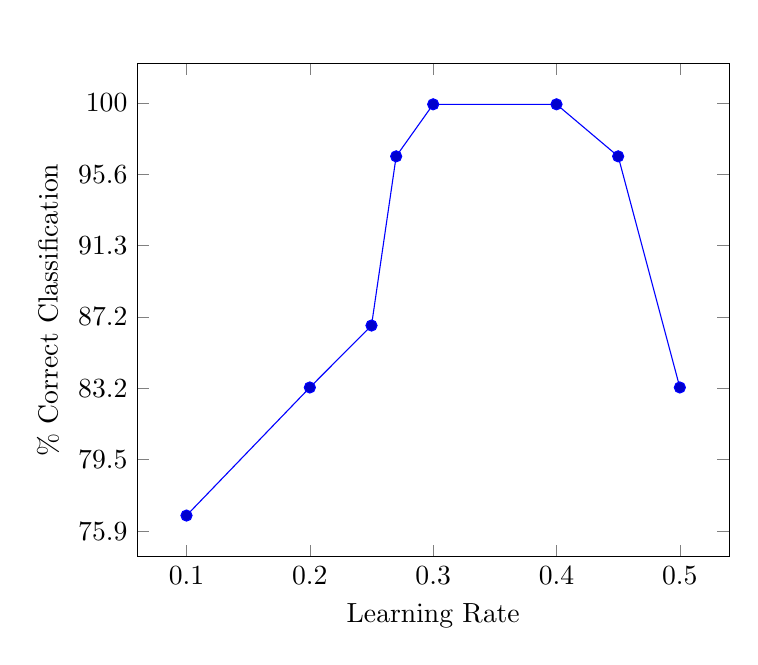
\begin{tikzpicture}
\begin{semilogyaxis}[title=\textbf{},
        scaled ticks=false,
        log ticks with fixed point,
    width=9.1cm,
        ylabel = \% Correct Classification,
        xlabel = Learning Rate
]
\addplot plot coordinates {(0.1, 76.7)(0.2,83.3)(0.25,86.7)(0.27, 96.7)(0.3, 100)(0.4,100)(0.45,96.7)(0.5,83.3)};
\end{semilogyaxis}
\end{tikzpicture}
\caption{graphical representation of figure 1 results}
\end{center}
\end{figure}
\paragraph{Results}
The data from my search for optimum $\alpha$ values is in figure 1. Looking at these it is clear that choosing a value too low or too high produces a bad result. This is
not surprising as a low learning rate makes the network learn very slowly while a high learning rate makes the weights and objective function diverge, so there is no learning 
at all. Starting out from $\alpha = 0.1$, I then stopped at $\alpha = 0.5$ as this produced a great decrease in accuracy\\\\
The best value I found was between [ $0.3 \rightarrow 0.4$ ]. Over my ten tests for each of these values, they both produced a perfect classification. As seen in figure 2, the upper 
$\alpha$ value produced the greater decrease (steepest slope) so I chose 0.3 as my optimum value.
\paragraph{Conclusion} 
Over the course of my experiment I found that I needed different starting values for my bias and weights. This was done to minimise the occurrence of multiple perceptrons firing.
I also found that it was valuable to do ten tests of each setting for the learning rate due to the fact that I was choosing random values at the beginning of each test. Averaging the
results then gave me some insight into the true performance of that setting. \\\\
Finally, I found that $\alpha =  0.3$ was my optimum value and produced best results. I should also mention that for 10 tests of $\alpha = 0.3$, only one caused a "winner takes all" 
situation as opposed to 4 instances where $\alpha = 0.5$.

\bibliographystyle{plain}

\end{document}